% ================================================================
% CHAPTER 1: Ausgangslage
% ================================================================


\chapter{Ausgangslage}

\section{Beschreibung der Situation }

In den letzten Jahren ist die Landwirtschaft zunehmend unter Druck geraten. Der Primärsektor verliert an volkswirtschaftlicher Bedeutung \cite[S. 1  f.]{Hofer}. Sowohl der Anteil an Beschäftigten als auch die landwirtschaftliche Nutzfläche sinkt \citep[S. 2 ]{Hofer} und Preise für Agrarprodukte sind stark unter Druck \citep[S. 11 ]{Hofer}. Daraus entsteht ein tiefgreifender Strukturwandel \cite[S. 11  f.]{Hofer}. Zahlreiche Landwirte gehen Nebentätigkeiten nach, um zusätzliches Einkommen zu generieren \citep[S. 6]{Hofer}. Deshalb stellen sowohl die Maximierung des landwirtschaftlichen Einkommens als auch die Ermöglichung der Nutzung von Nebenerwerbsquellen besondere Herausforderungen in der Landwirtschaft dar \citep[S. 8]{Stefan2003}. Für selbstständige Landwirte ist es nicht einfach, einem Nebenerwerb nachzugehen.


Auch der Landwirt Peter Müller geht einer Nebenerwerbstätigkeit nach und will daher im landwirtschaftlichen Betrieb\footnote{Standort des Betriebs: Schwellibach 50, CH-1714 Heitenried, Kanton Freiburg} nach innovativen Lösungen suchen, welche der Doppelbelastung entgegenwirken \citep{Muller2019}. \\


\begin{figure}[H]
	\center
	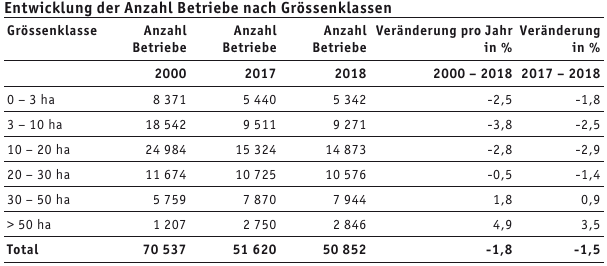
\includegraphics[scale=0.72]{Grafiken/Betriebsstatistik.PNG}
	\caption{Entwicklung der Anzahl Haupt- und Nebenerwerbsbetriebe nach Regionen \citep{Unbekannta}} 
	\label{fig: Entwicklung der Anzahl Haupt- und Nebenerwerbsbetriebe nach Regionen}
\end{figure}


Um möglichst viel Milch zu produzieren, sorgen Landwirte dafür, dass jede Kuh auf dem Bauernhof einmal pro Jahr ein Kalb gebärt. Bei 15 Kühen auf dem Bauernhof des Arbeitgebers bedeutet dies mehr als eine Geburt pro Monat \citep{Muller2019}.

Jede Geburt, bei welcher der Landwirt abwesend ist, könnte  für die Kuh und das Kalb ein lebensbedrohliches Risiko darstellen \citep{Muller2019}. 

Dieser Bezug zur Problemstellung hat der Autor im Rahmen der Case-Arbeit \flqq{}Technologische Unterstützung von Landwirten bei der Geburt von Kälbern und bei der Heuernte\frqq{} erarbeitet. Es wurde ein System entwickelt, welches in regelmässigen zeitlichen Abständen Kamerabilder aufnimmt und auf einer Website darstellt. Das System zeigt Kamerabilder in passender Qualität zwecks Beobachtung auf einer Website an. Ziel dieses Systems ist die automatische Unterstützung mit Benachrichtigung auf verschiedenen Kommunikationskanälen bei der Überwachung. Damit wird das Risiko bei der Geburt von Kälbern und das Risiko von Schäden an der Infrastruktur zur Heuernte reduziert.


Sowohl Dr. med. vet. Samuel Kohler\footnote{Kontakt per E-Mail: \url{samuel.kohler@bfh.ch}}, Tierarzt und Studiengangsleiter Agronomie bei der BFH (HAFL) und Prof. Dr. med. vet. Gaby Hirsbrunner\footnote{Kontakt per E-Mail: \url{gabriela.hirsbrunner@vetsuisse.unibe.ch}} vom Departement für klinische Veterinärmedizin der Universität Bern als auch der Auftraggeber, der Landwirt Peter Müller\footnote{Postadresse: Schwellibach 50, 1714 Heitenried}, sehen die Case-Arbeit als spannende Lösung mit Optimierungspotential. Zurzeit müssen die aufgenommenen Kamerabilder von Landwirten nach wie vor auf einer Website angezeigt und von Menschen interpretiert werden. Die computergetriebene, vollautomatische Verarbeitung und Analyse von Kamerabildern stellt eine sinnvolle Weiterentwicklung zur Reduzierung des Überwachungsaufwands dar. 

\section{Bedarf}

Dystokie ist die Todesursache von $50$ bis $66$ Prozent der Kalbsgeburten mit tödlichem Ausmass. Dies hat auch wirtschaftliche Konsequenzen in Form von Kosten für die Dienstleistungen des Tierarztes, nicht verkauften Kälbern, tieferer Milchproduktion oder vorzeitiger Schlachtung. Darüber hinaus ist Dystokie schmerzvoll und beeinträchtigt das Wohlergehen der Kühe \citep[S. 1]{Saint-Dizier2015}. Die Geburt ist ein kritisches Ereignis für Kuh und Kalb und oftmals Auslöser für nachfolgende Krankheiten. Optimales Management und Überwachung der Geburt wirken diesen Risiken entgegen und vermindern die Eintrittswahrscheinlichkeit von Dystokie und Totgeburt \citep[S. 1]{Lange2017}. Die Prognose des Geburtszeitpunkts unterstützt die Entscheidung, ob und wann menschliche Geburtshilfe angebracht ist. Die Unterstützung beim Abkalben bewirkt eine Verringerung der Kälbersterblichkeit und der \gls{Plazenta}-\gls{Retention}. Die Vorhersage des Geburtszeitpunkts ist daher sowohl für die Wirtschaftlichkeit der Tierhaltung als auch für das Wohlergehen der Tiere von Bedeutung \citep[S. 1]{Saint-Dizier2015}.  


Zum heutigen Zeitpunkt gibt es diverse Lösungsansätze zur Analyse des Geburtsverlaufs. Neigungs- und Beschleunigungssensoren sollen die Schwanzhebung und Verhaltensänderungen erkennen \citep[S. 6]{Saint-Dizier2015}. Zudem können spezialisierte Wiederkäuersensoren, welche beispielsweise von der Forschungsanstalt Agroscope\footnote{Weitere Informationen zu Agroscope: \url{https://www.agroscope.admin.ch}} entwickelt werden, das Wiederkäuerverhalten der Tiere analysieren \citep[S. 2]{Pahl2014}. Intelligente Bauchgürtel sind gemäss \citep[S. 6]{Saint-Dizier2015} in der Lage, \gls{Abdominal}kontraktionen zu detektieren. Intravaginale Sensoren erkennen einen Abfall der Körpertemperatur und die Ausstossung des \gls{Allantochorions}\footnote{siehe Glossar}. Zudem gibt es Vorrichtungen in der Vagina oder an den Schamlippen, welche die Ausstossung der Waden erkennen. Sämtliche Produkte funktionieren nach demselben Prinzip: Sobald ein Sensor das prädiktive Merkmal erkennt, wird dieses analysiert und eine Benachrichtigung an den Landwirten ausgelöst. So wird der Landwirt vor dem bevorstehenden Abkalben gewarnt. Die wissenschaftliche  Basis der angebotenen Produkte ist  jedoch oftmals mangelhaft. Diese Einschätzung von \citep[S. 6]{Saint-Dizier2015} hat mehrere Ursachen. Einerseits berücksichtigen die Produkte oftmals nur eine geringe Anzahl von Parametern zur Analyse. Andererseits bringt zurzeit keines der getesteten Geräte die Möglichkeit, Dystokie oder die Notwendigkeit menschlicher Geburtsunterstützung zu erkennen. Ausserdem wurden die meisten Studien bei der Rasse Holstein\footnote{ \url{https://www.swissherdbook.ch/unsere-rassen/holstein-red-holstein/}}\textsuperscript{,}\footnote{\url{https://swissgenetics.com/genetik/rassenspezifische-informationen/holstein/}} in Milchkuhhaltung durchgeführt. Sowohl in der Sammlung von Erfahrungen bei anderen Rassen als auch anderer Haltung liegt grosses Verbesserungspotential. Dementsprechend ist die Einführung von technischen Systemen zur Sammlung von Daten bei einer grossen Anzahl von Tieren anstrebenswert. So können weitere Wissenquellen gewonnen werden, welche für die Entwicklung von erfolgreicheren Produkten nützlich sind \citep[S. 6]{Saint-Dizier2015}. Die vorliegende Arbeit beinhaltet die Analyse von Kamerabildern während der Geburt von Kälbern der Rasse Swiss Fleckvieh\footnote{\url{https://swissgenetics.com/genetik/rassenspezifische-informationen/swiss-fleckvieh/}}\textsuperscript{,}\footnote{\url{https://www.swissherdbook.ch/unsere-rassen/swiss-fleckvieh/}}. Dadurch kann die Arbeit einen Beitrag zum Gewinn von weiteren Erfahrungen in dieser Domäne leisten.

In der Studie von \cite[S. 6]{Ouellet2016} wurden 42 Kühe mit Sensoren ausgestattet, wobei acht davon die Sensoren verloren haben und durch technische Probleme mit dem Wiederkäuersensor bei zwei weiteren Kühen keine Daten zum Wiederkäuerverhalten gesammelt werden konnten. Der Einsatz von Kameras hingegen ermöglicht eine sichere Entfernung zwischen Kuh und technischer Einrichtung. Der Autor ist der Meinung, dass diese Entfernung die Ausfallsicherheit des System erhöhen kann. Um den optimalen Abstand zwischen Kamera und Tieren festzulegen, wurden die empirischen Versuche durch Angaben der Tierärzten überprüft und dementsprechend angepasst.
 
\section{Ziele }

Wünschenswert ist nun, im Rahmen der Bachelor-Thesis ein System zu entwickeln, welches die automatische Analyse von Kamerabildern zur Prognose des Geburtszeitpunkts von Kälbern ermöglicht.

Der Aufwand für die Überwachung des Geburtsverlaufs ist auf ein Minimum reduziert, weil die Lösung vollständig digitalisiert ist.

Dieses System soll modular und erweiterbar sein und optimalerweise auch in der Lage sein, Landwirte und Tierärzte mittels direkter und gezielter Benachrichtigungen fast in Echtzeit über den Geburtsverlauf von Kälbern zu informieren. Grundlage für diese Benachrichtigung bildet die computergetriebene Analyse von Bildmaterial.

Im Rahmen der vorliegenden Bachelor-Thesis wird zwischen Projektzielen (A), betrieblichen (B) und optionalem Zielen (C) unterschieden.


\textbf{Projektziele (Ziele zum Lieferergebnis)}

\begin{table} [H]
	
	\rowcolors{2}{maroon!10}{white!100}
	\arrayrulecolor{darkmaroon} 
	
	\begin{tabular}{ p{1cm} p{14cm} }
				
		\toprule[1pt]
		\rowcolor{maroon!30}	
		ID & Beschreibung \\
		
		\midrule 
		A1 & Das System liest Bilddateien von einem vorgegebenen Dateisystem ein.\\		
		A2 & Das System bearbeitet die von der Kamera gelieferten Bilder.\\				
		A3 & Das System arbeitet auf Basis von geometrischen Mustern und visuellen Merkmalen unter Berücksichtigung gegebener, konfigurierbarer Schwellwerte. \\		
		A4 & Das System arbeitet aus sicherer Entfernung zu den Tieren, sodass es nicht invasiv ist.\\				
		A5 & Das System ist durch anerkannte Prinzipien des Software-Engineerings so aufzubauen,
		dass eine beliebige technische Komponente ausgetauscht werden kann und die
		neue Implementierung für die restlichen Schichten keine Auswirkung hat.\\		
		
		\bottomrule
	\end{tabular}
	\caption{Projektziele}
	\label{tab: Projektziele}
\end{table}

\newpage

\textbf{Ziele im Betrieb}


Die folgende Tabelle verdeutlicht die betrieblichen Ziele im Zusammenhang mit der Geburt von Kälbern.

\begin{table}[H]
	\rowcolors{2}{maroon!10}{white!100}
	\arrayrulecolor{darkmaroon} 
	
	\begin{tabular}{ p{1cm} p{14cm} }
		
		\toprule[1pt]
		\rowcolor{maroon!30}	
		ID & Beschreibung \\
		
		\midrule 
		B1 & Das System reduziert den Aufwand für die manuelle Überwachung des Geburtsverlaufs dank Kamerabildern. \\
		B2 & Das System stellt sowohl für Landwirte als auch Tierärzte ein digitales Werkzeug zur Entscheidungsunterstützung zur Verfügung.\\
		B3 & Das System senkt Geburtsrisiken für Kuh und Kalb. Dies erhöht die Wirtschaftlichkeit der Tierhaltung und das Wohlergehen der Tiere. \\
		B4 & Das System vereinfacht die Einleitung von gezielten Massnahmen zur Geburtshilfe.\\
		\bottomrule
		
	\end{tabular}
	\caption{Betriebliche Ziele für die Überwachung bei der Geburt von Kälbern.}
	\label{tab: Betriebliche Ziele für die Überwachung bei der Geburt von Kälbern.}
\end{table}

\textbf{Optionale Ziele }

Folgende Tabelle verdeutlicht die anstrebenswerten Ziele, welche einen zusätzlichen Mehrwert erschaffen sollen.
\begin{table}[H]
	\rowcolors{2}{maroon!10}{white!100}
	\arrayrulecolor{darkmaroon} 
	
	\begin{tabular}{ p{1cm} p{14cm}  }
		
		\toprule[1pt]
		\rowcolor{maroon!30}		
		
		ID & Beschreibung \\
		
		\midrule 
		C1 & Das System erkennt Bilder bei welchen in den nächsten 12 Stunden noch keine Geburt stattfindet und löst daraufhin eine vordefinierte, konfigurierbare Aktion aus. In einer ersten Phase handelt es sich um eine konfigurierbare Meldung, die in der Konsole der Entwicklungsumgebung ausgegeben wird.\\ 
		C2 & Das System ist in der Lage, Landwirte und Tierärzte mittels Benachrichtigungen als Nachricht über Kommunikationskanäle wie ) SMS, b) Twitter, c) WhatsApp oder d) Mail über den Geburtsverlauf von Kälbern zu informieren.  \\
		\bottomrule
		
	\end{tabular}
	\caption{Optionale Ziele für die Überwachung bei der Geburt von Kälbern.}
	\label{tab: Optionale Ziele für die Überwachung bei der Geburt von Kälbern.}
\end{table}
